%%
%% The first command in your LaTeX source must be the \documentclass command.
%% nonacm option turns off ACM stuff like copyright notice and such
\documentclass[sigplan,screen,nonacm]{acmart}

%%
%% \BibTeX command to typeset BibTeX logo in the docs
\AtBeginDocument{%
  \providecommand\BibTeX{{%
    \normalfont B\kern-0.5em{\scshape i\kern-0.25em b}\kern-0.8em\TeX}}}

% painint TODOs red    
\newcommand\TODO[1]{\textcolor{red}{\emph{TODO #1}}}

% for line break inside table cells
% t c or b for desired vertical alignment
\newcommand{\specialcell}[2][t]{%
  \begin{tabular}[#1]{@{}l@{}}#2\end{tabular}}

\usepackage{tikz}
\usetikzlibrary{arrows.meta}

\usepackage[ruled, linesnumbered]{algorithm2e}
% \usepackage{algorithmic}
\renewcommand{\b}{\boldsymbol}

%Path relative to the main .tex file 
% path to the images folder
\graphicspath{{./img/}}
\usepackage{subcaption}

\setlength{\parskip}{0.2em}

%% end of the preamble, start of the body of the document source.
\begin{document}
% don't allow lines to overflow their columns
% \sloppy

% \renewcommand{\@algocf@capt@plain}{top} % formerly {bottom}
%%
%% The "title" command has an optional parameter,
%% allowing the author to define a "short title" to be used in page headers.
\title[Hair Simulation]{Simulation of Curly Hair}
\subtitle{5th Semester Project Laboratory Report}

%%
%% The "author" command and its associated commands are used to define
%% the authors and their affiliations.
%% Of note is the shared affiliation of the first two authors, and the
%% "authornote" and "authornotemark" commands
%% used to denote shared contribution to the research.
\author{Barnabás Börcsök}
% \authornote{BSc student}
\email{borcsok.barnabas@simonyi.bme.hu}
\affiliation{%
  \institution{}%Budapest University of Technology and Economics}
  \city{}
  \country{}
}

\author{Dr. László Szécsi}
\email{Advisor}
\affiliation{%
    % \institution{Budapest University of Technology and Economics}
    % \city{}
    % \country{}
    % \department[0]{Computer Graphics Group}
    % \department[1]{Department of Control Engineering and Information Technology}
    \institution{}
    \city{}
    \country{}
}


%%
%% By default, the full list of authors will be used in the page
%% headers. Often, this list is too long, and will overlap
%% other information printed in the page headers. This command allows
%% the author to define a more concise list
%% of authors' names for this purpose.
% \renewcommand{\shortauthors}{Trovato and Tobin, et al.}

%%
%% The abstract is a short summary of the work to be presented in the
%% article.
\begin{abstract}
    A self-assessment of the 5th semester Project Laboratory
    Project is presented in this article. My goal was to achieve hair simulation
    of acceptable quality both in terms of look and performance. Multiple
    approaches were considered before arriving at a Position Based Dynamics
    based solution. The simulation was implemented in C++ with the Open Graphics
    Library (OpenGL \footnote{\url{http://www.opengl.org}}). 
\end{abstract}

%%%
%%% The code below is generated by the tool at http://dl.acm.org/ccs.cfm.
%%% Please copy and paste the code instead of the example below.
%%%
\begin{CCSXML}
<ccs2012>
<concept>
<concept_id>10010147.10010371.10010352.10010379</concept_id>
<concept_desc>Computing methodologies~Physical simulation</concept_desc>
<concept_significance>300</concept_significance>
</concept>
</ccs2012>
\end{CCSXML}

\ccsdesc[300]{Computing methodologies~Physical simulation}
%%
%% Keywords. The author(s) should pick words that accurately describe
%% the work being presented. Separate the keywords with commas.
\keywords{hair simulation, position based dynamics, OpenGL}

%% A "teaser" image appears between the author and affiliation
%% information and the body of the document, and typically spans the
%% page.
\begin{teaserfigure}
  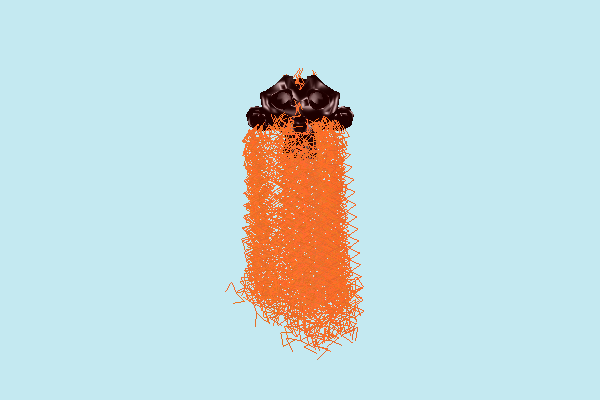
\includegraphics[width=\textwidth]{teaser.png}
  \caption{The achieved visual look}
  \Description{Using 400 hair pieces, with 25 particles on each piece of hair.}
  \label{fig:teaser}
\end{teaserfigure}

%%
%% This command processes the author and affiliation and title
%% information and builds the first part of the formatted document.
\maketitle
\renewcommand{\shortauthors}{Barnabás Börcsök}


\section{Introduction}
In the 5th semester of their undergrad studies, BSc students from Budapest
University of Tehchnology and Economics embark on their first journey of
scientific research. I was always interested in and fascinated by computer 
graphics, it came naturally to choose a subject in this area. As I had little
 hands-on experience in this field, a long time had to be dedicated
to research and trying out different simulation methods.

The first part of this paper reflects this, giving an overview of considered
methods, and other possible routes that could have been taken to implement hair
simulation.


The implementation and all of the code mentioned is available at
\url{http://git.sch.bme.hu/bobarna/brave-2}.

\section{Overview of considered methods}

There were mainly three methods considered, two of them being substantially
different:


\subsection{Mass Spring System}
The whole idea of doing hair simulation as my project laboratory came after
reading \citet{PixarPaper}. They outline a method for the artistic simulation of
curly hair for use in their film production. The method was featured in the 2012
movie Brave.

This approach models the hair as a chain of particles with given mass, each
connected via springs. This results in a mass-spring system, which is then
modeled by considering well-known physics formula's such as Newton's second law
of motion $F=m*a$, and Hooke's Law, which states that the force $F$
needed to extend or compress a spring by some distance $x$ scales linearly with
respect to that distance. The paper by \citet{PixarPaper} created an elaborate
system of springs, with additional core springs making the simulation stable
and resulting in the desired look and feel.

The main characteristic of this approach is that a Mass Spring System deals with
forces, and tries to stay true to the laws of physics. It accounts for internal 
and external forces from which accelerations are computed based on Newton's 
second law of motion. A time integration method is then used to update the
velocities and finally the positions of the particles. This will not be the case
with Position Based Dynamics.
\subsection{Position Based Dynamics (PBD)}

The paper by \citet{MullerPBD} presents an approach that omits the velocity as
well as the force layer of the then-present popular approaches for simulation
methods of dynamic systems in computer graphics.

Position Based Dynamics (PBD) -- as its name suggests -- works with the position
of particles. A big advantage of such a system lies in its controllability, and
the easy reducability of overshooting problems present in force based systems.
Another favorable aspect is that PBD methods are generally easier with the maths
and somewhat easier to implement in terms of the needed mathematical and
physical background needed to grasp its inner workings. In addition, -- as it
works directly with the position of particles -- collision constraints can be
handled easily and penetrations can be resolved completely by projecting points
onto the penetrated surface. Although such measures can only be applied on the
expanse of physical accuracy, position based dynamics being only a ``good
enough'' approximation of how objects behave in real life.

Chapter 2 of the paper by \citet{UmenhofferSimulation} builds on the
\citet{MullerPBD} paper and gives a concise overview of the position based
dynamics method, and goes on to show the type of constraints that can be applied
to control to behaviour of such a system -- which is present in both papers.


\subsection{Follow-the-Leader (FTL)}
The Dynamic Follow-the-Leader (FTL) method outlined by \citet{FTLHair} focuses
on the fast simulation of hair and fur on animated characters. The sheer number
of computation needed for simulating thousands of hair strands, each consisting
of numerous particles presents a big challenge. Also, as each strand is
inextensible, it is not trivial to come up with an algorithm that does its job
in feasible time. 

As it will be covered later in this article, the already introduced PBD method
needs multiple iterations per frame in order to keep the system from stretching
and becoming unstable. The FTL method by \citet{FTLHair} presents a method that
takes only a single iteration through the particles of each hair strand per
frame to achieve the desired results.

As this sounds fascinating, and cuts the computation time needed substantially,
in the early stages of my project, I implemented the FTL method alongside PBD.
It \textit{works}, and is fast, although due to the iteration count being one,
when greater forces are being applied to the system, a substantial amount of
stretching was introduced to the system. As it seemed in comparison that the
``basic'' PBD method yielded the same -- or even more accurate -- results, and
it was feasible to allow myself to use multiple iterations per frame, I did
not further investigate if there could have been improvements made to my
implementation to eliminate the stretching in the presence of greater forces.


\section{Position Based Simulation}

\subsection{Algorithm Overview}
\label{section:algorithmOverview}
We model an $S$ hair strand as a chain of $N$ particles and a set of $M$
constraints. Each particle $p \in [1,\ldots,N]$ has three attributes: mass ($m_p$), position
($\boldsymbol{x_p}$) and velocity ($\boldsymbol{v_p}$). 

A constraint $c \in [1,\ldots,M]$ with cardinality $n_c$ is a function $C_c
: \mathbb{R} ^{3n_c} \mapsto \mathbb{R}$. It operates on a set of indices $\{i_1,\ldots
i_{n_c}\}, i_k \in [1,...,N]$. The constraint function also has a stiffness
parameter $k_c \in [0...1]$ and a type of either \emph{equality} or
\emph{inequality}.

Constraint $c$ with type \emph{equality} is satisfied if
$C_c(\boldsymbol{x}_{p_1},\ldots, \boldsymbol{x}_{p_{n_j}})=0$. If its type is
\emph{inequality}, then it is satisfied if $C_c(\boldsymbol{x}_{p_1}, \ldots,
\boldsymbol{x}_{p_{n_c}}) \geq 0$. The stiffness parameter $k_c$ defines the
strength of the constraint in a range from zero to one.

Given these notations, the algorithm works in the following way:

\begin{algorithm}
    \caption{pseudo code for the PBD simulation}\label{alg:pbd}

    \SetCommentSty{scriptsize}
    \SetNlSty{texttt}{(}{)}

    % to turn off vertical lines:
    % \SetAlgoNoLine

    \SetKwBlock{Loop}{loop}{end}

    \SetKwFunction{dampVelocities}{dampVelocities}
    \SetKwFunction{genCollCon}{generateCollisionConstraints}
    \SetKwFunction{projCon}{projectConstraints}
    \SetKwFunction{velUpdate}{velocityUpdate}

    \SetKwProg{loopTimes}{loop}{ times}{end loop}

    \ForEach{p in particles}{ 
        initialize $\b{p_x} = \b{x_p^0}, \b{p_v} = \b{v_p^0}, p_w = 1/m_p$ 
    }

    \Loop{
        \ForEach{p in particles}{
            $\b{p_v} \gets \b{p_v} + \Delta t \cdot p_w \cdot \b{f_{external}}$
        }
        \dampVelocities{$p_1, \ldots, p_N$}
        \\
        \ForEach{p in particles}{
            $\b{p_{tmp}} \gets \b{p_x} + \Delta t \cdot \b{p_v}$

        }
        \ForEach{p in particles}{
            \genCollCon{$p_x \to p_{tmp}$}
        }
        \loopTimes{numberOfIterations}{
            \projCon{$C_1,\ldots, C_{M+M_{coll}}, particles$}\\
            \tcc*[f]{only the temporary positions of $particles$ are needed}
        }
        \ForEach{p in particles}{
            $\b{p_v} \gets (\b{p_{tmp}} - \b{p_x})/\Delta t$\\
            $\b{p_x} \gets \b{p_{tmp}}$
        }
        \velUpdate{$particles$}\\
        \tcc*[f]{velocities of colliding particles are modified according to
        friction and restitution coefficients.}
    }
\end{algorithm}

\newcommand{\lineRef}[2]{{\footnotesize\texttt{(#1)}-\texttt{(#2)}}}
\newcommand{\lineRefSingle}[1]{{\footnotesize\texttt{(#1)}}}

Lines \lineRef{1}{3} initialize the particles. We store the inverse masses $w$
in order to be able to store infinitely heavy particles that are stationary
during the simulation. ($\frac{1}{\infty} \approx 0$)

The core idea of position based dynamics is shown in lines \lineRef{9}{11},
\lineRef{15}{17} and \lineRef{18}{21}. In line \lineRefSingle{10}, estimated
positions for each particle $\b{p}$ are calculated using and explicit forward
Euler integration step. In line \lineRefSingle{16} the iterative solver manipulates
these temporary position estimates such that they satisfy the constraints. It
does this by repeatedly projecting each constraint in an iterative manner to
similar to that of a Gauss-Seidel
\footnote{\url{https://en.wikipedia.org/wiki/Gauss\%E2\%80\%93Seidel\_method}}
solver \emph{(see section \ref{sec:solver})}. Once the solver finishes with the
iterations, in lines \lineRef{19}{20} each particle is moved to the calculated
(once temporary) positions, and the velocity of each particle is updated
accordingly.

Velocities are manipulated in lines \lineRefSingle{6}, \lineRefSingle{8} and
\lineRefSingle{19}. 

Line \lineRefSingle{6} allows to account for external forces
in the simulation if some of the forces cannot be converted to positional
constraints. \emph{(For example the pulling force between subsequent particles
are modeled as distance constraints instead of external forces, and so are the
forces generated by the particles colliding with other objects.)} We use it to
add gravity, and to generate wind effects for demonstration purposes. If only
the gravitational force is present, then the line becomes $\b{p_v} \gets \b{p_v}
+ \Delta t \cdot \b{g}$, where $\b{g}$ is the gravitational acceleration.

In line \lineRefSingle{8} the velocities can be damped, if necessary. \emph{Section
3.5} of the \citet{MullerPBD} paper gives some more sophisticated methods for
damping, although the paper also points out that any form of damping can be
used. In our case, simply applying a $k_s$ damping coefficient with value
between $98\%$ to $99.9\%$ seemed to be a good enough solution.

The initial constraints $C_1, \ldots, C_M$ are fixed throughout the simulation.
In addition to these initial constraints, line \lineRefSingle{13} generates additional
$M_{coll}$ collision constraints. These change from time step to time step. The
projection step in line \lineRefSingle{16} considers both the fixed and the
collision constraints. Our implementation does not yet utilize this opportunity
to dynamically generate collision constraints. This is one of the possible future
works outlined in the subsection \nameref{subsec:future_work_collision}.

\subsection{The Solver}
\label{sec:solver}
The input to the solver are $M + M_{coll}$ constraints and the temporary
($\b{p_{tmp}}$) positions of the particles. The aim of the solver is to modify
the estimates such that they satisfy all the constraints. This yields a system
of equations. For solving these for particle positions we use
a sequence of Gauss-Seidel-type iterations. The original Gauss-Seidel algorithm
can only handle linear systems, although we have a non-linear system of
equations of hand. Even a simple distance constraint $ C(\b{p_1}, \b{p_2})
= \lvert \b{p_1} - \b{p_2} \rvert - d $ yields a non-linear equation. In
addition, the constraints of type \emph{inequality} yield inequalities.

The part we borrow from the Gauss-Seidel method is the idea of solving each
constraint independently one after the other. This makes up the essence of the
method: we repeatedly iterate through all the constraints and project the
particles to valid locations with respect to the given constraint alone.
Modifications to point locations immediately get visible to the process. This
speeds up convergence significantly, because pressure waves can propagate
throughout the chain of particles in a single solver step, and effect which is
dependent on the order in which constraints are solved. 

In our hair simulation case, we solve the distance constraints by putting the
hair particles at the desired distance from each other starting at the scalp,
and moving outwards from there.

For projecting the constraints, we utilize the method proposed by
\citet{MullerPBD}. The details of computing the desired delta positions are
explained in Appendix \ref{appendix:ConstraintProjection}
\nameref{appendix:ConstraintProjection}. An example derivation is given in
Section \ref{section:DistanceConstraint} \nameref{section:DistanceConstraint}.

There are several ways of incorporating the stiffness parameter. The simplest
-- and the way we chose to utilize -- is simply multiplying the $\Delta \b{p}$
correction by the $k \in [0 \ldots 1]$ stiffness parameter. For multiple
iteration loops of the solver, the effect of $k$ becomes non-linear. The
remaining error after $n_s$ solver iterations is $\Delta \b{p}(1-k)^{n_s}$.
\citet{MullerPBD} propose to multiply the corrections not by $k$ directly, but
by $k' = 1 - (1-k)^{1/n_s}$. With this transformation, the error becomes $\Delta
\b{p}(1-k')^{n_s} = \Delta\b{p}(1-k)$, and thus linearly dependent on $k$ and
independent of $n_s$. The resulting stiffness is still dependent on the time
step of the simulation. Real time environments typically use fixed time steps in
which case this dependency is not problematic.

\subsection{Distance Constraint} \label{section:DistanceConstraint}
One of the most basic constraint is the Distance Constraint, forcing two given
particles $d$ distance apart. It is an \emph{equality} type constraint, meaning
that it is satisfied if $C_{distance} = 0$.

\begin{equation} \label{eq:distance_constraint}
C_{distance}(\b{p_1},\b{p_2}) = \lvert \b{p_1} - \b{p_2} \rvert - d
\end{equation}
We are looking for $\Delta \b{p_1}$ and $\Delta \b{p_2}$ corrections such that 
$$
C_{distance}(\b{p_1}+\Delta \b{p_1}, \b{p_2}+\Delta \b{p_2}) = 0.
$$

In finding the desired delta values to satisfy the constraint, we follow the
method proposed by \citet{MullerPBD} \emph{(see Appendix
 \nameref{appendix:ConstraintProjection})}.

The derivatives with respect to the positions are
\begin{align*}
    \nabla_{\b{p_1}} C_{distance}(\b{p_1}, \b{p_2}) &= \b{n} \\\\
    \nabla_{\b{p_2}} C_{distance}(\b{p_1}, \b{p_2}) &= -\b{n} \\\\
    \b{n} = \frac{\b{p_1}-\b{p_2}}{\lvert \b{p_1}-\b{p_2} \rvert}.
\end{align*}
This makes the scaling factor 
\begin{align*}
    s &= \frac{C(\b{p_1},\b{p_2})}
{w_1 \lvert \nabla_{p_1}C(\b{p_1}, \b{p_2})\rvert ^ 2 + w_2 \lvert
\nabla_{p_2}C(\b{p_1}, \b{p_2})\rvert ^ 2}\\\\
    &= \frac{\lvert \b{p_1} - \b{p_2}\rvert - d}{w_1 + w_2}.
\end{align*}
The final corrections are:
\begin{align*}
    \Delta \b{p_1} &= - \frac{w_1}{w_1 + w_2}
    (\lvert \b{p_1} - \b{p_2} \rvert - d) 
    \frac{\b{p_1} - \b{p_2}}{\lvert \b{p_1} - \b{p_2} \rvert} 
    \\\\
    \Delta \b{p_2} &= + \frac{w_2}{w_1 + w_2}
    (\lvert \b{p_1} - \b{p_2} \rvert - d) 
    \frac{\b{p_1} - \b{p_2}}{\lvert \b{p_1} - \b{p_2} \rvert}
\end{align*}

\begin{figure}
    % \rule{\columnwidth}{0.05em}
    \label{fig:dist_constr_proj}
    \caption{Projection of the distance constraint $C(\b{p_1}, \b{p_2}) = \lvert \b{p_1}
    - \b{p_2} \rvert - d$. The corrections $\Delta \b{p_i}$ are weighted according
    to the inverse masses $w_i = 1/m_i$.}
    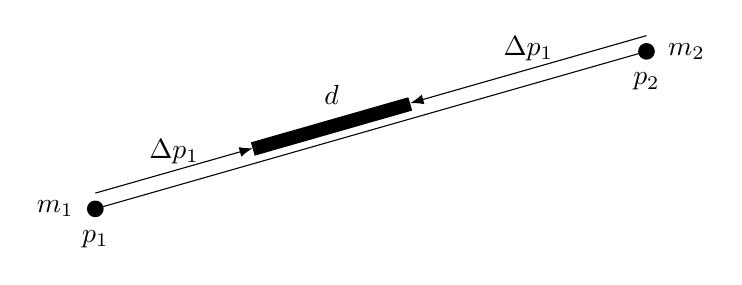
\begin{tikzpicture}
        
        \draw[-] (-3,0)--(4,2);
         
        % p1 in lower left
        \fill[black] (-3,0) circle (0.7ex);
        \draw (-3,0) node[below=1ex]{$\b{p_1}$};
        \draw (-3,0) node[left=1ex]{$m_1$};

        \draw[-Latex] (-3,0.2) -- (-1,0.77);
        \draw (-2,0.3) node[above=1ex]{$\b{\Delta \b{p_1}}$};
        
        % p2 in upper right
        \fill[black] (4,2) circle (0.7ex);
        \draw (4,2) node[below=1ex]{$\b{p_2}$};
        \draw (4,2) node[right=1ex]{$m_2$};

        \draw[Latex-] (1,1.343) -- (4,2.2);
        \draw (2.5,1.6) node[above=1ex]{$\b{\Delta \b{p_1}}$};

        % middle
        \draw[line width=0.5em] (-1,0.76) -- (1,1.333);
        \draw (0,1.0465) node[above=1ex]{$d$};
        
    \end{tikzpicture}
    % \rule{\columnwidth}{0.05em}
\end{figure}

Since the type of the Distance Constraint is \emph{equality}, the projection is
straight forward: we move both by $\b{p_1}$ and $\b{p_2}$ by $\Delta \b{p_1}$ and
$\Delta \b{p_2}$ respectively.

\subsection{Bending Constraint} \label{section:bendingConstraint}
\citet{UmenhofferSimulation} use the PBD technique to simulate cloth materials.
They utilize the bending constraint to define the bending resistance of the
material, giving it an extra stiffness. Their goal with the Bending Constraint
is to keep an initial angle between adjacent triangles formed by particles. They
offer the $C(p_1,p_2,p_3,p_4) = arccos(n_1 \cdot n_2) - \phi _0$ constraint,
where $n_1$ and $n_2$ are the normal vectors of the triangles, and $p_2 - p_1$
forms the common side of the two triangles. The $\phi _0$ angle is measured
between the normals of the two triangles.

At first, we thought about implementing something similar for our project, but
then simplified the ``Bending Constraint'' for our use-case to essentially
 distance constraints $C_{distance}(p_{i-1}, p_{i+i})~for~i\in[1 \ldots
n_{particles}-1]$ of the same hair strand with the $d$ distance paramter of the
being lower than the $d$ parameter of other $C_distance$ constraints keeping the
particles a given $l_{seg}$ distance apart from each other, and assigning
a lower $k_{bending}$ stiffness parameter.

This idea could be further developed when considering other $(p_j,p_k)$ pairs
and different distances between them. Figure \ref{fig:bendingConstraint}
illustrates some example variety in the behaviour of chain of particles under
different bending constraints.

\newcommand{\simulationDetails}[3]{\emph{$nr_{seg}=#1$, $l_{seg}=#2$, $k=#3$}}
\begin{figure*}
    \caption{Different distance and particle pairing definitions yield
    significantly different results. Particle masses were slightly randomized
    for a variance between strands. In each below simulation, $nr_{seg}$
    particles of length $l_{seg}$ were generated. Distance constraints acting as
    bending constraints had a stiffness parameter $k$. Distance
    constraints responsible for keeping the particles $l_{seg}$ distance apart
    always had a $k_{pos}=1$ stiffness parameter.}
    \label{fig:bendingConstraint}
    \begin{subfigure}{.5\linewidth}
        \caption{\simulationDetails{120}{0.005}{0.6}}
        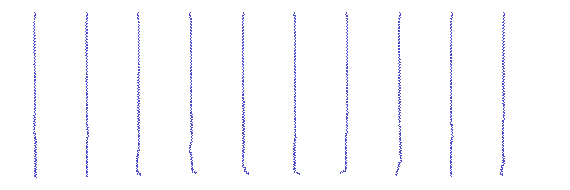
\includegraphics[width=\linewidth]{bend_con_10Sim_120Seg_0.005lSeg.png}
    \end{subfigure}%
    \begin{subfigure}{.5\linewidth}
        \caption{\simulationDetails{60}{0.01}{0.6}}
    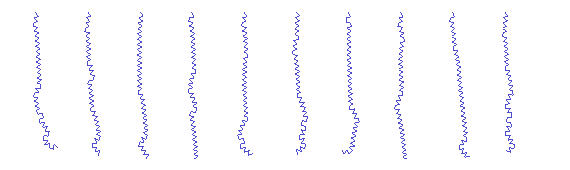
\includegraphics[width=\linewidth]{bend_con_10Sim_60Seg_0.01lSeg.png}
    \end{subfigure}%
    \par\medskip
    \begin{subfigure}{.5\linewidth}
        \caption{\simulationDetails{30}{0.02}{0.6}}
    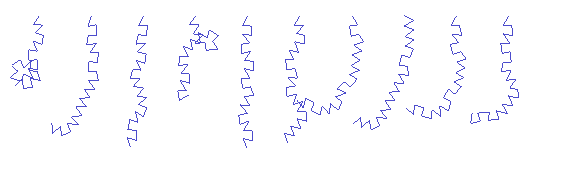
\includegraphics[width=\linewidth]{bend_con_10Sim_30Seg_0.02lSeg.png}
    \end{subfigure}%
    \begin{subfigure}{.5\linewidth}
        \caption{A distance constraint between the first and last particles
        were given. \simulationDetails{40}{0.015}{0.8}}
    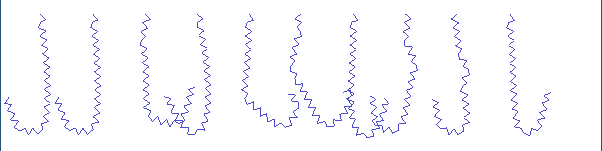
\includegraphics[width=\linewidth]{bend_con_first_last_10Sim_40Seg_0.015lSeg.png}
    \end{subfigure}%
\end{figure*}

\subsection{Collision Constraint}
One huge advantage of the position based approach is how simply collision
handling can be realized. In each simulation step $M_{coll}$ collision
constraints are generated in the \lineRef{12}{14} lines of Algorithm
\ref{alg:pbd}. For a moving particle $\b{p}$ and points $\b{q_1}, \b{q_2},
\b{q_3}$ forming a triangle with normal $\b{n}$, the collision constraint is

$$
C_{collision}(\b{p}, \b{q_1}, \b{q_2}, \b{q_3}) = (\b{p}-\b{q_1})\cdot \b{n} \geq 0
$$

, where we check whether $\b{p}$ lies on the desired side of the given
surface. We require that the magnitude of the vector from an arbitrary point
on the surface to $\b{p}$ projected onto the normal vector be greater than 0 by
utilizing the dot product operation.

The formula for solving the triangle collision constraint is:

$$
\Delta \b{p_{tmp}} = -((\b{p_{tmp}}-\b{q_1})\cdot \b{n})\cdot \b{n}
$$

This formula moves the particle along the triangle normal exactly to the
triangle's surface. 

\subsection{Position Constraint}
Maybe the most straight-forward constraint is the Position Constraint, given as:
\begin{align*}
    C_{collision}(\b{p}) &= \lvert \b{p} - \b{p_{goal}} \rvert = 0
    \\
    \Delta \b{p} &= \b{p_{goal}} - \b{p}
\end{align*}

Moving the $\b{p}$ particle to the $\b{p_{goal}}$ position.

We utilize the Position Constraint for keeping the first particle in each strand
on the surface of the head.


\section{Implementation}
After introducing the general position based dynamics simulation method, we dive
into the specifics we settled on for our hair simulation.

The code is available at \url{http://git.sch.bme.hu/bobarna/brave-2}.

\subsection{Data Structures}

The properties of particles introduced in chapter
\ref{section:algorithmOverview} \nameref{section:algorithmOverview} got an
additional color property. This decision was made so hair with a gradient color
could be simulated.

\begin{verbatim}
    class Particle {
        vec3 pos;
        vec3 tmp;
        float w;
        vec3 v;
        vec3 color;
    }
\end{verbatim}

The strands are stored as a vector of vector of Particles. It is practical to
keep related data packed right after each other in the memory for improving the
performance of operations and function calls.


\subsection{Constraints}
A \texttt{Constraint} class with an abstract \texttt{solve()} method was
implemented, storing each derived constraint class \emph{(e.g.
PositionConstraint, BendingConstraint)} in a heterogeneous
collection and calling each overriden \texttt{solve()} method when projecting
the constraints in the iteration loop (line \lineRefSingle{16} of Algorithm
\ref{alg:pbd}).

This implementation proved to be not fast enough, lagging even with low particle
counts. We could not discover the cause of this increased computational time, and
decided to settle on another solution. Instead of the above mentioned, we
store only the parameters that constraints operate on, and the simulation calls
the relevant solve functions with these stored parameters.


\subsection{Putting the Hair in the Hair Simulation}
The $PBDSimulation$ class handles the simulation and rendering of the hair. It
takes a $HeadObject$ and propagates hairstrands starting from its surface. Each
strands first particle is fixed in place with a $PositionConstraint$, not
letting it move away from the scalp.

The geometry of the $HeadObject$ is read from an \texttt{OBJ} file. (\emph{See
the Appendix \ref{section:appendixOBJ} \nameref{section:appendixOBJ}}.)

The hair strands are propagated throughout the surface of the $HeadObject$ by
proposing random $(\b{u}, \b{v}) \in [0 \ldots 1] \times [0 \ldots 1]$
coordinates and settling on them if they satisfy requirements for the position
of the hair -- like the corresponding face in world coordinates has an upward
pointing normal vector. This propagation of strands on the surface of the head
could be improved, as pointed out in sections
\nameref{section:futureCustomization} and \nameref{section:futureHalton}.
 

\section{Results}
The implementation is available at \url{git.sch.bme.hu/bobarna/brave-2}. The
program is able to handle up to around 500 individual hair strands, each
consisting of around 30 particles in real time. With the implemented OBJ reader,
it is possible to achieve diverse visual results in no time.

An example result shown in Figure \ref{fig:teaser}, and can
be seen in the supplementary videos
\href{https://drive.google.com/drive/folders/1n79xSokrBe2lKQixX_DacF7wByXkbpZP?usp=sharing}{available
here}.\footnote{\url{https://drive.google.com/drive/folders/1n79xSokrBe2lKQixX_DacF7wByXkbpZP?usp=sharing}}
An 8-minute video was also made to supplement this writing. It is accessible at
\TODO{link to 8-minute video}

\section{Conclusion}
\label{sec:conclusion}
After investigating and trying out multiple methods to simulate hair, we arrived
at the Position Based Dynamics (PBD) method. An overview of the PBD method, and
an introduction to the constraint types used in our implementation was given.
An implementation was made in C++ and OpenGL, which easily simulates the hair
strands in real time, although the limit of the real-time method can easily be
surpassed when adding around a thousand strands each with more than 30
particles.

\section{Future Work}
\label{sec:future_work}
As this was part only of a semester-long Project Laboratory course, a great deal
of time was dedicated in the early stages of the project to investigate and
explore the subject area. This left only a sub-optimal time for implementing all
desired aspects of the simulation.

\subsection{Hair-hair Collisions}
\label{subsec:future_work_collision}
As it is computationally expensive to simulate each particle colliding with all
of the other particles, a particle density field could be used. One such method
of grouping hair particles and their corresponding velocities into a 3D voxel
grid is outlined in the paper by \citet{PixarVolumetricHair}, which was also
utilized in the \citet{FTLHair} paper for handling hair-hair collisions.
Such a method could be used to dynamically generate collision constraints in
line \lineRefSingle{13} of Algorithm~\ref{alg:pbd}.

\subsection{Bending Constraint Improvements}
As already mentioned in Section \ref{section:bendingConstraint}
\nameref{section:bendingConstraint}. A huge improvement could be made by
improving the bending constraint either by further exploring the possibilities
of defining different distance constraints between pairs of particles.

An alternative route could be to explore the possibility of a different type of
bending constraint, for example by keeping a given angle between chunks of
subsequent particles.

\subsection{More and better customization} 
\label{section:futureCustomization}
A drawable texture map is considered for the ability to tell the simulation
where to put the hair strands on the surface of the head.

The \texttt{OBJ} reader could also be further developed into reading material,
texture and/or color data for the objects.

A common interface for importing and exporting different hairstyles could be
developed.

\subsection{Better customizability}
In the current implementation there is no way to properly customize the look and
feel of the hair without accessing the source code. A possible improvement could
be to read material and texture data for the hair from the OBJ file. Another
huge improvement could be to set the constraints in real time, giving the user
much better control of the hair. Other properties, such as length of the hair
segments and color of the hair could be set as well.

\subsection{Sequence for randomizing hair positions}
\label{section:futureHalton}
In the current implementation, a standard C++ random number generator is
utilized. Utilizing a low-discrepancy number sequence such as the Halton
sequence for randomizing hair strand positions would be an improvement.

\subsection{Rendering}
This semester left no time to try out different methods for rendering and
visualizing the hair. The current implementation connects the individual
particles with GL\_LINES, resulting in a sub-optimal visual experience. Offline
(e.g. ray-tracing) methods could utilize the current simulation method. 
The paper by \citet{RappRealTime} discusses the real-time aspect of hair
rendering in great detail, supplemented with a broad discussion on different
parts of the (OpenGL) rendering pipeline that could be utilized.

\subsection{Moving to the GPU}
The current implementation runs solely on the CPU. A big leap forward would be
the utilization of the GPU. Compute shaders for computations are considered. The
paper by \citet{UmenhofferSimulation} discusses a parallelization of the
different constraint solves, although as they work on the same dataset, some
computation problems are present during the parellelization of the
problem.

Tesselation and geometry shaders could be utilized for the rendering and display
of the particles, resulting in a far better image with the same simulation
method and properties.

%%
%% The acknowledgments section is defined using the "acks" environment
%% (and NOT an unnumbered section). This ensures the proper
%% identification of the section in the article metadata, and the
%% consistent spelling of the heading.
\begin{acks}
    To Dr. László Szécsi, associate professor at the Computer Graphics Group
    (Department of Control Engineering and Information Technology), whom I had
    the chance to consult with during the semester.
\end{acks}

%%
%% The next two lines define the bibliography style to be used, and
%% the bibliography file.
\bibliographystyle{ACM-Reference-Format}
\bibliography{references}

%%
%% If your work has an appendix, this is the place to put it.
\appendix

\section{Constraint Projection} \label{appendix:ConstraintProjection}
Projecting a set of points according to a constraint means moving the points
such that they satisfy the constraint. As we move the points in the
simulation loop directly, the most important issue is the conservation of linear and
angular momentum. Let $\Delta \b{p_i}$ be the displacement of particle $i$ by the
projection. Linear momentum is conserved if 

\begin{equation}
    \label{eq:linear_momentum}
    \sum\limits_{i} m_i \Delta \b{p_i} = \b{0},
\end{equation}

which amounts to conserving the center of mass. Angular momentum is conserved if

\begin{equation}
    \label{eq:angular_momentum}
    \sum\limits_{i} \b{r_i} \times m_i \Delta \b{p_i} = 0,
\end{equation}

where the $\b{r_i}$ are the distances of the $\b{p_i}$ to an arbitrary common
rotation center. If a projection violates either the preservation of 
linear or angular momentum, \emph{ghost
forces} get introduced into the system, which act like external forces dragging
and rotating the object. However, only internal constraints need to conserve the
momenta. As we reduce the problem of collision handling to simply moving the
vertex to a valid point, it is somewhat trivial that for example collision
constraints are allowed to have global effects on the object.

The method that \citet{MullerPBD} propose conserves both momenta for internal
constraints. Let us look at a constraint $C$ with cardinality $n$ on the points
$\b{p_1}, \ldots, \b{p_n}$ with stiffness $k$. We let $\b{p}$ be the
concatenation $[\b{p_1}^T, \ldots, \b{p_n}^T]^T$. For internal constraints, $C$ is
independent of translation and rotation, which means that rotating or
translating the points does not change the value of the constraint function.
Therefore, the gradient $\nabla_{\b{p}} C$ is the direction of maximal change. If the
correction $\Delta \b{p}$ is chosen to be along $\nabla C_{\b{p}}$ both momenta
are automatically conserved if all masses are equal (we handle different masses
later). Given $\b{p}$ we want to find a correction $\Delta \b{p}$ such that
$C(\b{p}+\Delta\b{p})=0$. This equation can be approximated by

\begin{equation}
    C(\b{p}+\Delta\b{p}) \approx C(\b{p}) + \nabla_{\b{p}} C(p)\cdot\Delta
    p = 0.
    \label{eq:approximation}
\end{equation}

Restricting $\Delta \b{p}$ to be in the direction of $\nabla_{\b{p}}C$ means
choosing a scalar $\lambda$ such that

\begin{equation}
    \Delta{\b{p}} = \lambda \nabla_{\b{p}}C(\b{p}).
    \label{eq:restrictingLambda}
\end{equation}

Substituing Equation \ref{eq:restrictingLambda} into Equation
\ref{eq:approximation}, solving for $\lambda$ and subsituting back into Equation
\ref{eq:restrictingLambda} gives us the final formula for $\Delta\b{p}$:

\begin{equation}
    \Delta \b{p} = - \frac{C(\b{p})}{\lvert \nabla_{\b{p}} C(\b{p})\rvert^2}
    \nabla_{\b{p}}C(\b{p})
\end{equation}

which is a regular Newton-Raphson step for the iterative solution of the
non-linear equation given by a single constraint. For the correction of an
individual point $\b{p_i}$ we have

\begin{equation}
    \Delta \b{p_i} = -s\nabla_{\b{p_i}}C(\b{p_1},\ldots,\b{p_n}),
\end{equation}

where the scaling factor

\begin{equation}
    s = \frac{C(\b{p_1},\ldots,\b{p_n})}{
        \sum\limits_{j} \lvert\nabla_{\b{p_j}}C(\b{p_1},\ldots,\b{p_n})\rvert^2
    }
\end{equation}

is the same for all points. If the points have individual masses, we weight the
corrections $\Delta \b{p_i}$ by the inverse masses $w_i = 1/m_i$. In this case
a point with infinite mass, i.e. $w_i = 0$ for example does not move, just as
expected. Now Equation \ref{eq:restrictingLambda} is replaced by 
$$
\Delta \b{p_i} = \lambda w_i \nabla_{\b{p_i}}C(\b{p})
$$
yielding

\begin{equation}
    s = \frac{
        C(\b{p_1}, \ldots, \b{p_n})
    }{
        \sum\limits_{j}w_j\lvert\nabla_{\b{p_j}}C(\b{p_1},\ldots,\b{p_n})\rvert^2
    }
\end{equation}

for the scaling factor and for the final correction 

\begin{equation}
    \Delta \b{p_i} = -s w_i \nabla_{\b{p_i}}C(\b{p}).
\end{equation}


Section \ref{section:DistanceConstraint} gives an example by considering the
distance constraint function $C(\b{p_1},\b{p_2}) = \lvert\b{p_1}-\b{p_2}\rvert
- d$.


\section{Supplementary development}

\subsection{OBJ Reader}
\label{section:appendixOBJ}

An OBJ reader utility was implemented as part of the project. As the OBJ file
format \footnote{\url{http://paulbourke.net/dataformats/obj/}} describes a wide
range of properties for objects, our OBJ reader handles only the subset of these
description options -- those that are needed for the project. Unsupported line
types were simply ignored, still resulting in a successful file read if
possible.

\begin{table}[htb]
    \caption{Supported OBJ Data Types} 
    \label{tab:objdatatypes}
    % \begin{minipage}{\columnwidth}
        \begin{center}
            \begin{tabular}{ll}
                % \toprule
                Type of data & Format\\
                Comment & \# \verb|comment|\\
                Geometric vertex data & \verb|v x y z| \\
                Texture coordinates & \verb|vt u v| \\
                Vertex normals &\verb|vn i j k| \\
                Triangular faces &
                \specialcell{\texttt{f v1/vt1/vn1
                v2/vt2/vn2}\\\multicolumn{1}{r}{\texttt{... v3/vt3/vn3}}}\\
                % \bottomrule
            \end{tabular}
        \end{center}
    % \end{minipage}
\end{table}

\newcommand{\vFootNote}{\footnote{The obj file format allows for a w coordinate
(also called the weight) for describing rational curves and surfaces. The
default value of \textit{w} is 1.0. My implementation handles only the
assignment of \textit{x}, \textit{y} and \textit{z} values.}}

\newcommand{\vtFootNote}{\footnote{The obj file format allows for 3D texture
coordinates as well, but this implementation handles only 2D texture
coordinates.}}

\newcommand{\fFootNote}{\footnote{The obj file format allows for face
definitions far beyond only triangles, although this implementation handles only
face definitions of the above format.}}

\begin{itemize}
    \item ``\verb|v x y z|'' defines a vertex with position (x, y, z).\vFootNote 
    \item ``\verb|vt u v|'' defines a 2D texture coordinate with position (u,
        v).\vtFootNote 
    \item ``\verb|vn i j k|'' specifies a normal vector with components i, j and
        k.  
    \item ``\verb|f v1/vt1/vn1 v2/vt2/vn2 v3/vt3/vn3|'' Specifies a face with the
        given indices. For the first vertex, the \textit{v1}st previously
        defined vertex position is used, the \textit{vt1}st texture coordinate
        and \textit{vn1}st normal vector is used.\fFootNote
\end{itemize}


\subsection{Recording the simulation on-the-fly}
A recording utility was made to work in tandem with the application. In essence,
the rendered images are written into \texttt{bmp} or \texttt{png} files if the
capturing is enabled. In the
implementation\footnote{\url{https://git.sch.bme.hu/bobarna/brave-2}}, toggling
the capturing is mapped to the \texttt{C} key.


For handling the export of the rendered image into files, the
stb\_image\_write.h\footnote{\url{https://github.com/nothings/stb/blob/master/stb\_image\_write.h}}
single-file public domain library was used. 


The program outputs the image files in the \texttt{renders} folder at 24 FPS,
with the naming convention renderXXXX[.bmp/.png], where XXXX is the number of
the frame with left-padded zeroes.


After the image files are written, the user can start the
\texttt{make\_video.sh} script to assemble the \texttt{output.mp4} and delete
all the rendered frames. This script uses the free and open-source ffmpeg command
line utility\footnote{\url{https://ffmpeg.org/}}


\end{document}
\endinput
%%
%% End of file `documentation.tex'.
